% HET IP section

One major issue is to model correctly the instrumental profile (IP) of
\het. IP modeling is a crucial part of the precise RV work with iodine
calibration, as it affects directly several key procedures in the
Doppler pipeline, such as the creation of stellar spectrum template
and the forward-modeling of the observed stellar$+$iodine
spectrum. The current
successful IP model for Keck/HIRES (sum of Gaussians) in the CPS
pipeline is the product of careful studies and numerous trials with IP
modeling. A better understanding of the IP of HRS should bring visible
improvements to its RV precision. Finding a good IP for \het\ is also
an important exercise for modeling future fiber-fed precise RV
spectrographs, such as MINERVA, WIYN/NEID, and SHREK (on Keck).

How well the IP is being modeled can be tested by fitting an pure
iodine spectrum taken by the spectrograph
(Figure~\ref{het:fig:convkernel}). The typical $\chi_\nu^2$ value that
we obtain for fitting iodine spectra with a generic IP model
(Gauss-Hermite polynomials) is about 2.5, while for Keck/HIRES, the
$\chi_\nu^2$ value is typically around 1
(Figure~\ref{het:fig:iodchunkcomp}).


%----------------------------------------------------------------
% Demonstration of convolution to fit iodine atlas
% plot made by ~/Exo.../HET.../plots_general/convol_kernel/deconv_plot.pro
\begin{figure}
\centering
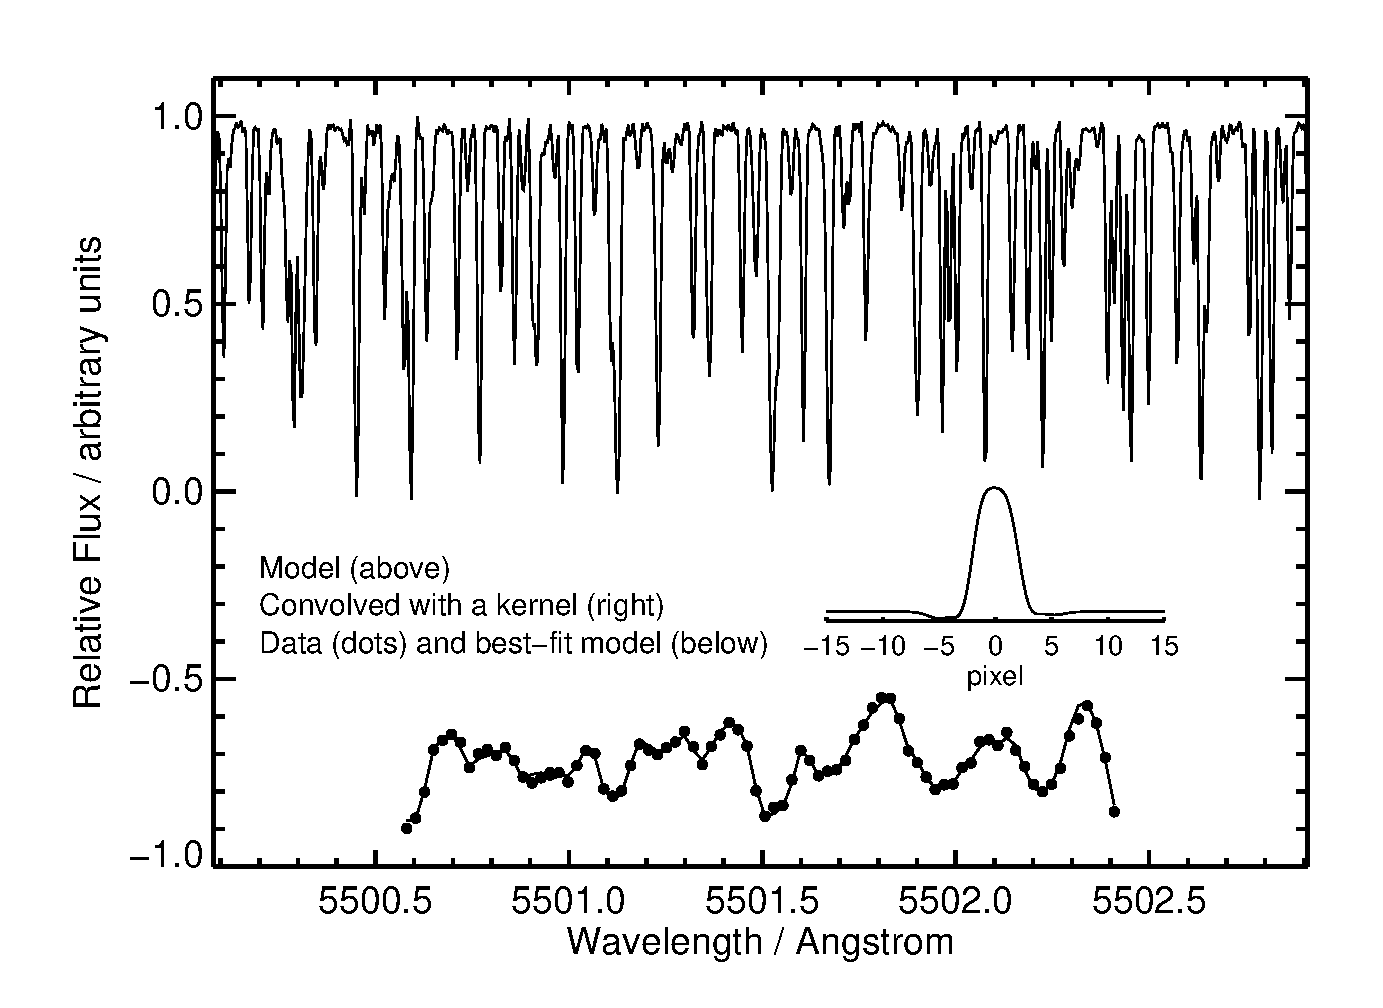
\includegraphics[scale=0.45]{het/convolution_kernel.eps}
\caption{Illustration of convolving the iodine atlas (sharp solid
  lines) with a kernel (middle right insert) to fit the observed
  iodine lines (black dots near the bottom, with best-fit model
  plotted in solid line).
\label{het:fig:convkernel}}
\end{figure}
%----------------------------------------------------------------



%----------------------------------------------------------------
% Comparison between HET and Keck chunk fit
% plot made by ~/Exo.../HET.../plots_general/fit_demo/plotfit.pro
\begin{figure}
\centering
\subfloat[\het\ Chunk]{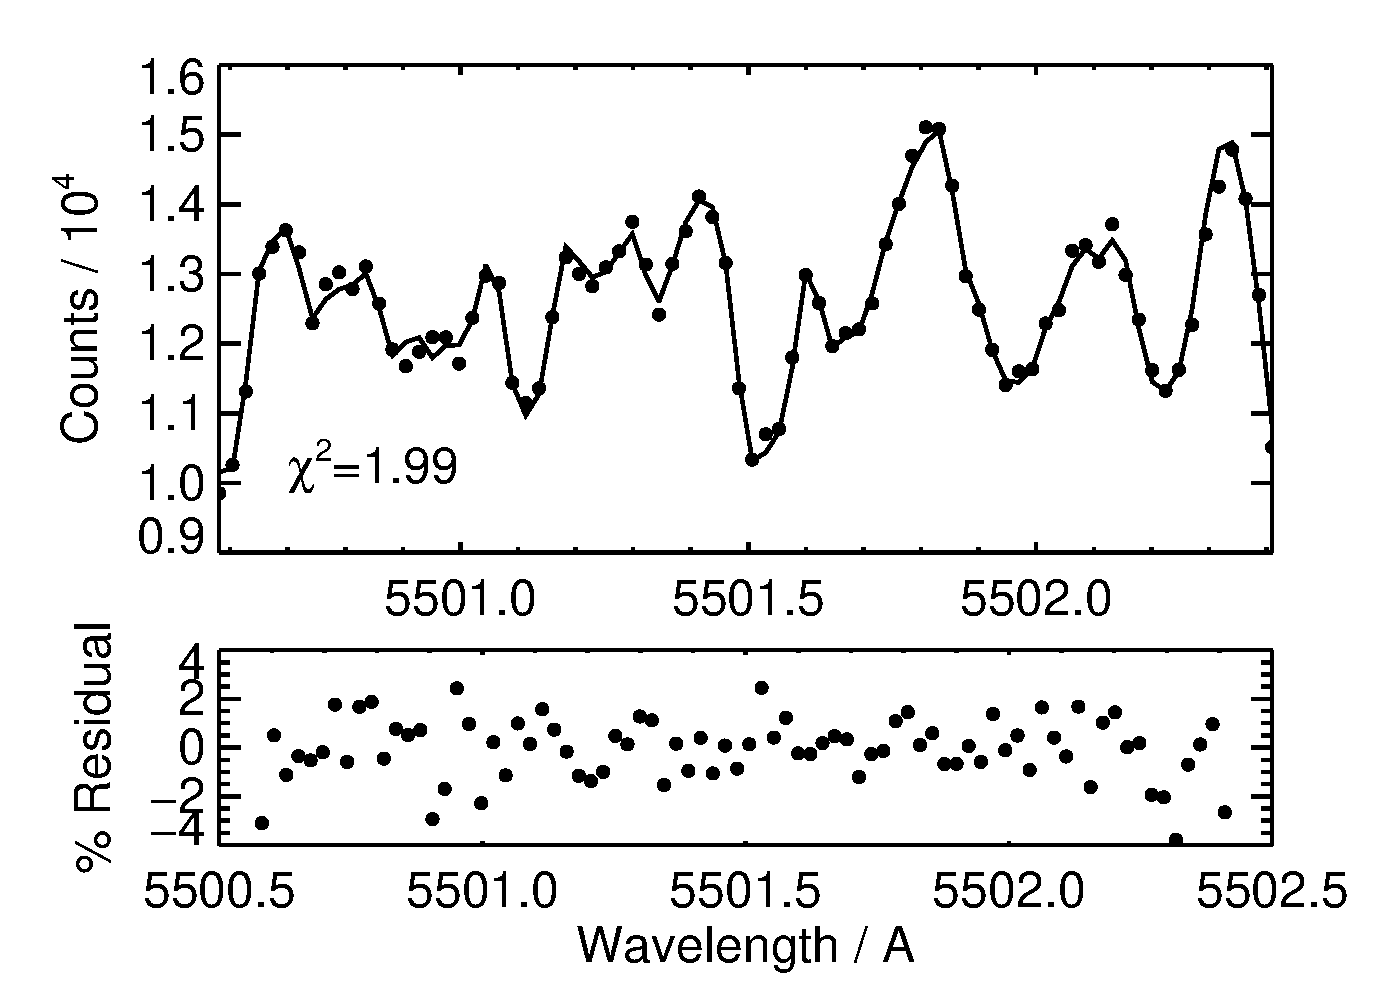
\includegraphics[scale=0.35]{het/20120124.176005.chunk189.eps}}
\subfloat[\keck\ Chunk]{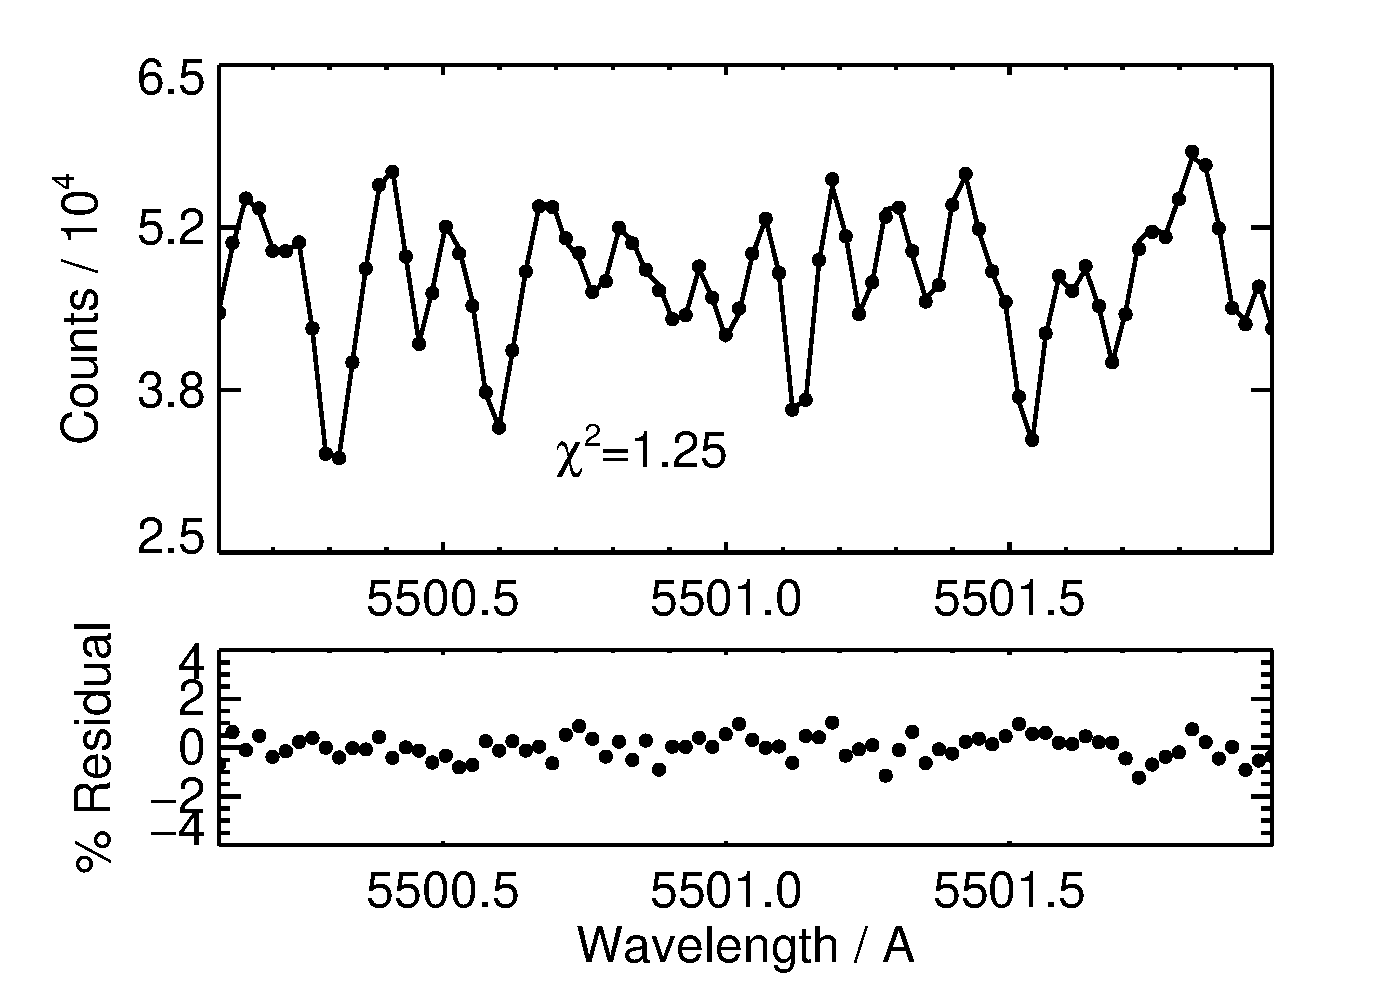
\includegraphics[scale=0.35]{het/rj82.77.chunk308.eps}}
\caption{Comparison between fits for a typical iodine-only chunk using
  \het\ data (left panel) and \keck\ data (right panel). Bottom panels
  are showing the residuals against best-fit models, plotted on the
  same $y$-axis scale. \het\ fit is significantly worse than \keck,
  which we believe is one of the major drivers behind \het's poorer RV
  precision. 
\label{het:fig:iodchunkcomp}}
\end{figure}
%----------------------------------------------------------------


The current ``go-to'' IP model for \hrs\ is the very versatile,
orthogonal, 11-parameter Gauss-Hermite polynomials (GH), which was
desribed in Chapter~\ref{chap:doppler}. Another customized IP for
\het\ was tried out by CPS, which was the sum of Gaussians, similar to
the one used for \keck\ but having the wings at different locations
with different default widths. The two IPs basically perform at a
similar level, with GH being slightly better
(Figure~\ref{het:fig:ghgau}). We have also tried several other
functional forms such as GH convolved with a top hat function with a
varying or fixed width, Lorentzian-Hermite (replacing the Gaussian in
GH with a Lorentzian), which all performed marginally worse than GH,
just like the sum of Gaussians. Or, more precisely, these IPs all seem
to be ``equally bad''.


%----------------------------------------------------------------
% Comparing 2005 and 2008 data, with GH and Gaussian IPs
% plot from ~/ExoPlanet-2010-2011/Professional_Development/201000-NSF_Jason/plots/
\begin{figure}
\centering
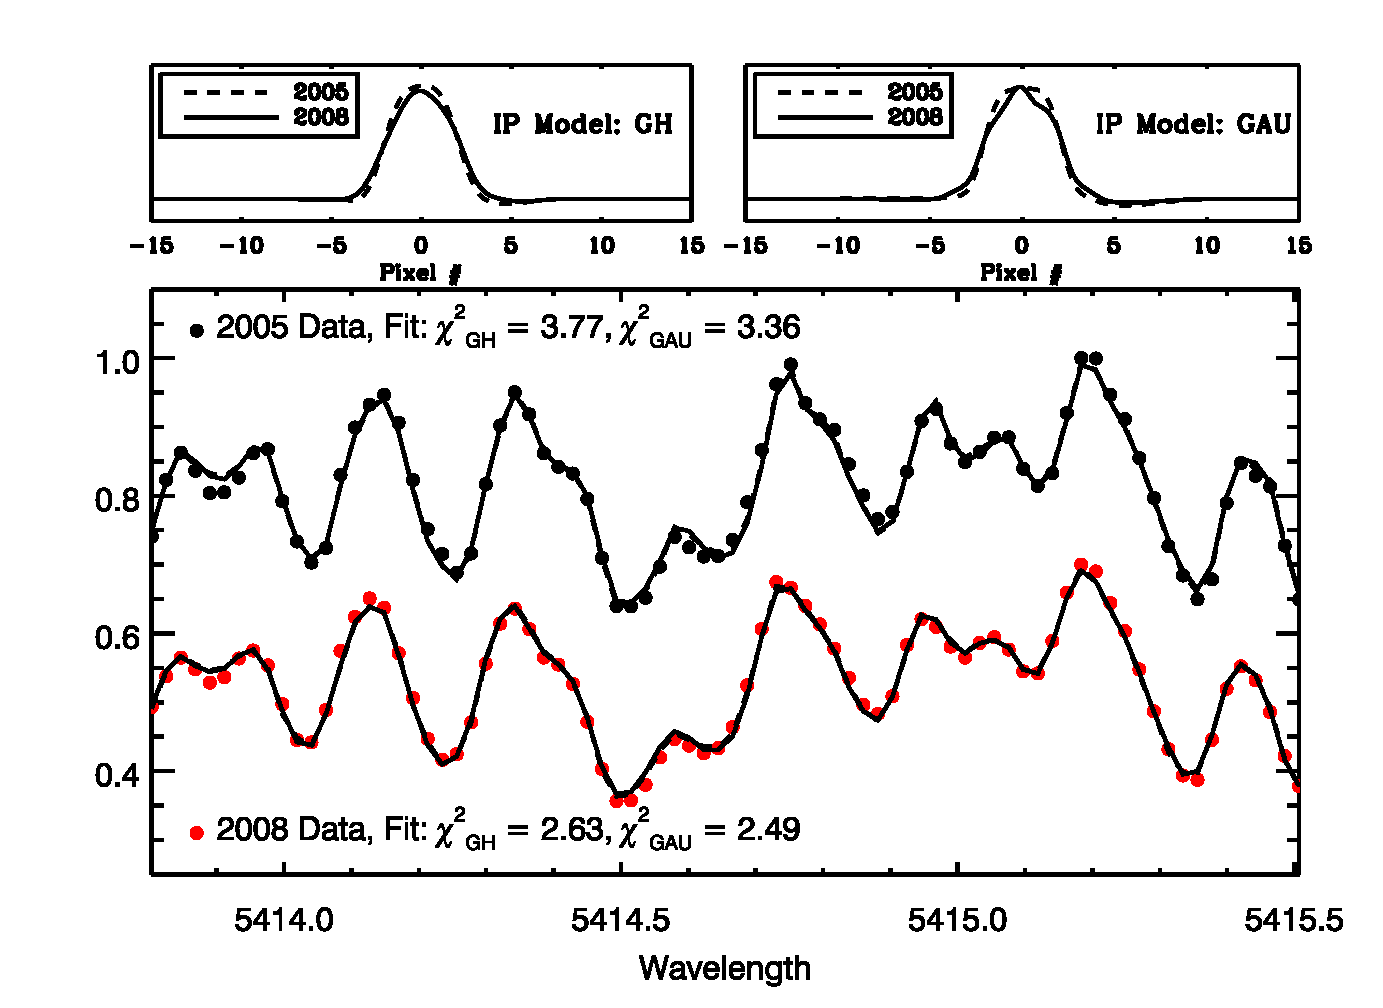
\includegraphics[scale=0.45]{het/iodfit.eps}
\caption{Illustration of fitting the iodine-only data (bottom panel)
  using different IPs (top panels), in this case, using GH and sum of
  Gaussians (GAU). These two IPs are practically ``equally bad",
  having similarly large reduced $\chi^2$ but neither produces a
  satisfactory fit. It is also interesting to see how ``stable" the
  best-fit IP can be across the years (i.e., in 2005 vs.~2008) and its
  smoothness, hinting that the best IP may take a simple, slowly-varying form. 
\label{het:fig:ghgau}}
\end{figure}
%----------------------------------------------------------------


We then looked at the Fourier space to see if that could provide some
clue. Figure~\ref{het:fig:fftip} plots the Fourier transform power
spectrum of the \het\ data (for the entire $\sim$1000\AA\ 1-D
extracted spectrum used for precise-RV purposes; with \keck\ data
also plotted for comparison). At high frequency in Fourier space, or
shorter periods in pixel space, i.e.\ on small scales, the power
spectrum is dominated by the signature of the IP. A ``null'' in the
power spectrum at 4.3 pixel is clearly visible, which suggests some
sort of sharp feature, and indeed, it exactly corresponds to the slit
width of \het\ at a resolution of R $=$ 60,000. This feature is a
direct result of the fact that HRS has the slit in front of a round
fiber, creating some what a sharp feature in its IP, unlike the
slit-fed \keck. 


%----------------------------------------------------------------
% Comparing Keck and HET IPs in Fourier space
% plot from screen shot of a slide in
% ~/ExoPlanet-2010-2011/Professional_Development/20150727-ThesisCommMeet/
% original plot is from ~/Exo../HET.../06-line.../powspec.pro and stored in ./plots/
\begin{figure}
\centering
\includegraphics[scale=0.45]{het/fftip.eps}
\caption{Fourier transform or power spectrum of a \het\ iodine-only
  spectrum (black dots) and its smoothed version (blue line). There is
  a clear signature of the \het\ slit at 4.3 pixel (corresponding to
  slit width for resolution R $=$ 60k). For comparison, the red curve
  is for \keck\ data, which shows no clear signiture of a slit,
  because \keck\ is not fiber-fed and the PSF of the star falls mostly
  within its slit.
\label{het:fig:fftip}}
\end{figure}
%----------------------------------------------------------------


Upon seeing the Fourier transform of the \het\ data, we tried out
another IP using GH multiplying a triangle (with a half width of 2.4
pixel and a height of 1), whose Fourier transform has a null at 4.3
pixel, and it produced the best fit among all IP models we have
ventured. Figure~\ref{het:fig:iodipcomp}, although it was perhaps
still ``equally bad''. At this point, we have already suspected that
the ``ground truth'' for the iodine lines, the iodine atlas, which was
created from a FTS scan, may be problematic. It would not be possible
to derive a correct form for the IP using a wrong iodine atlas, and
thus we shift our priority towards validating the iodine cell FTS and
investigating possible changes in the cell, which is described in the
next section.


%----------------------------------------------------------------
% Comparing fits with two IPs: GH, and GH+triangle
% plot made by ~/Exo.../HET.../plots_general/fit_demo/compfit.pro
\begin{figure}
\centering
\subfloat{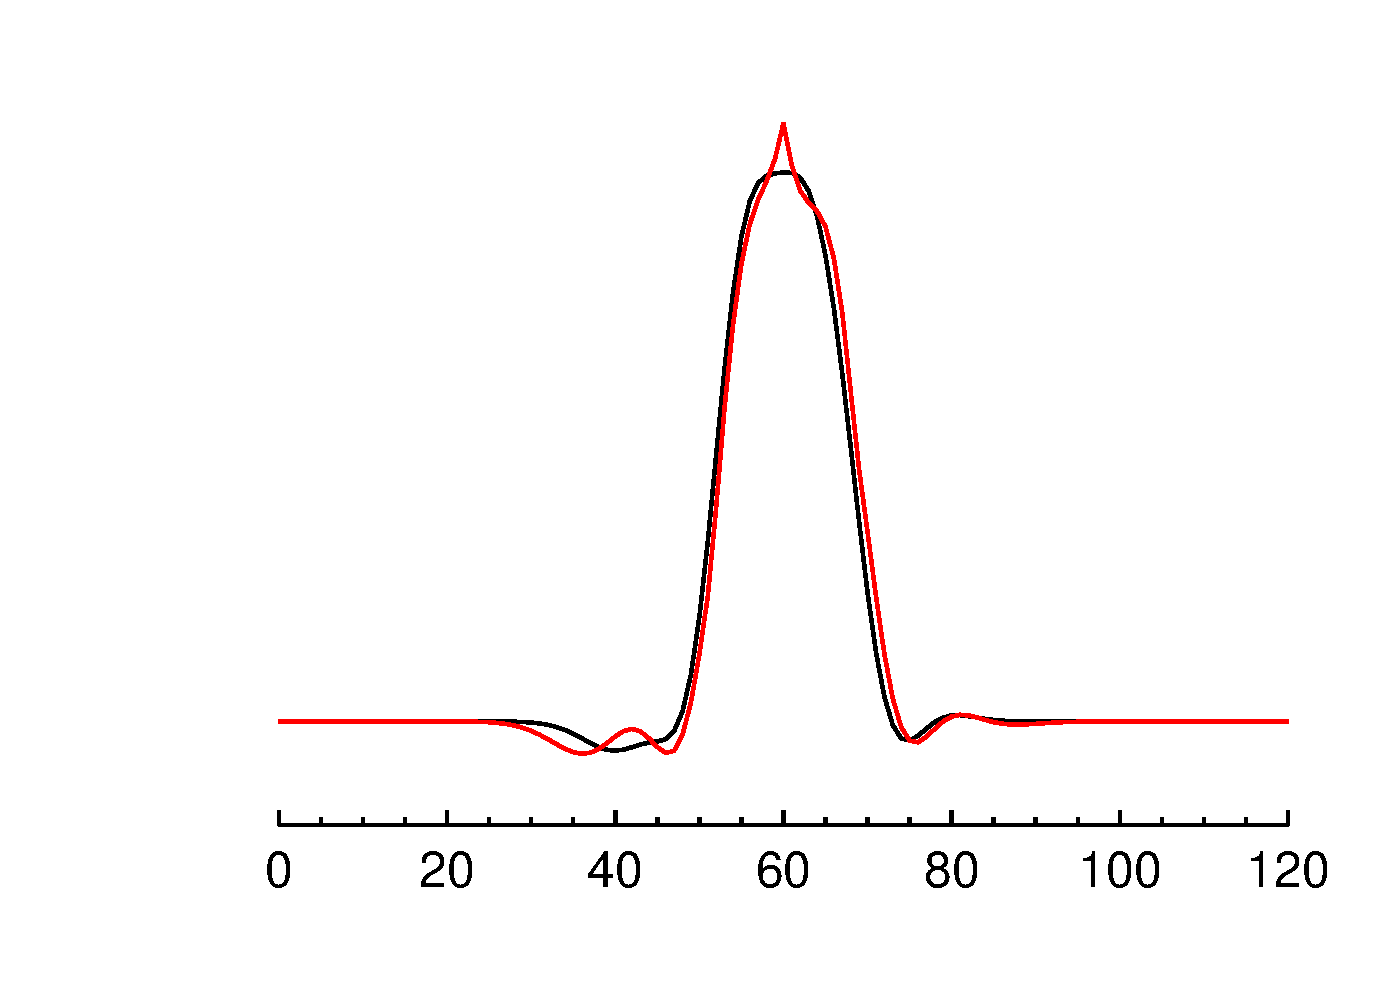
\includegraphics[scale=0.3]{het/20120124.176005.chunk191.compip.eps}}
\subfloat{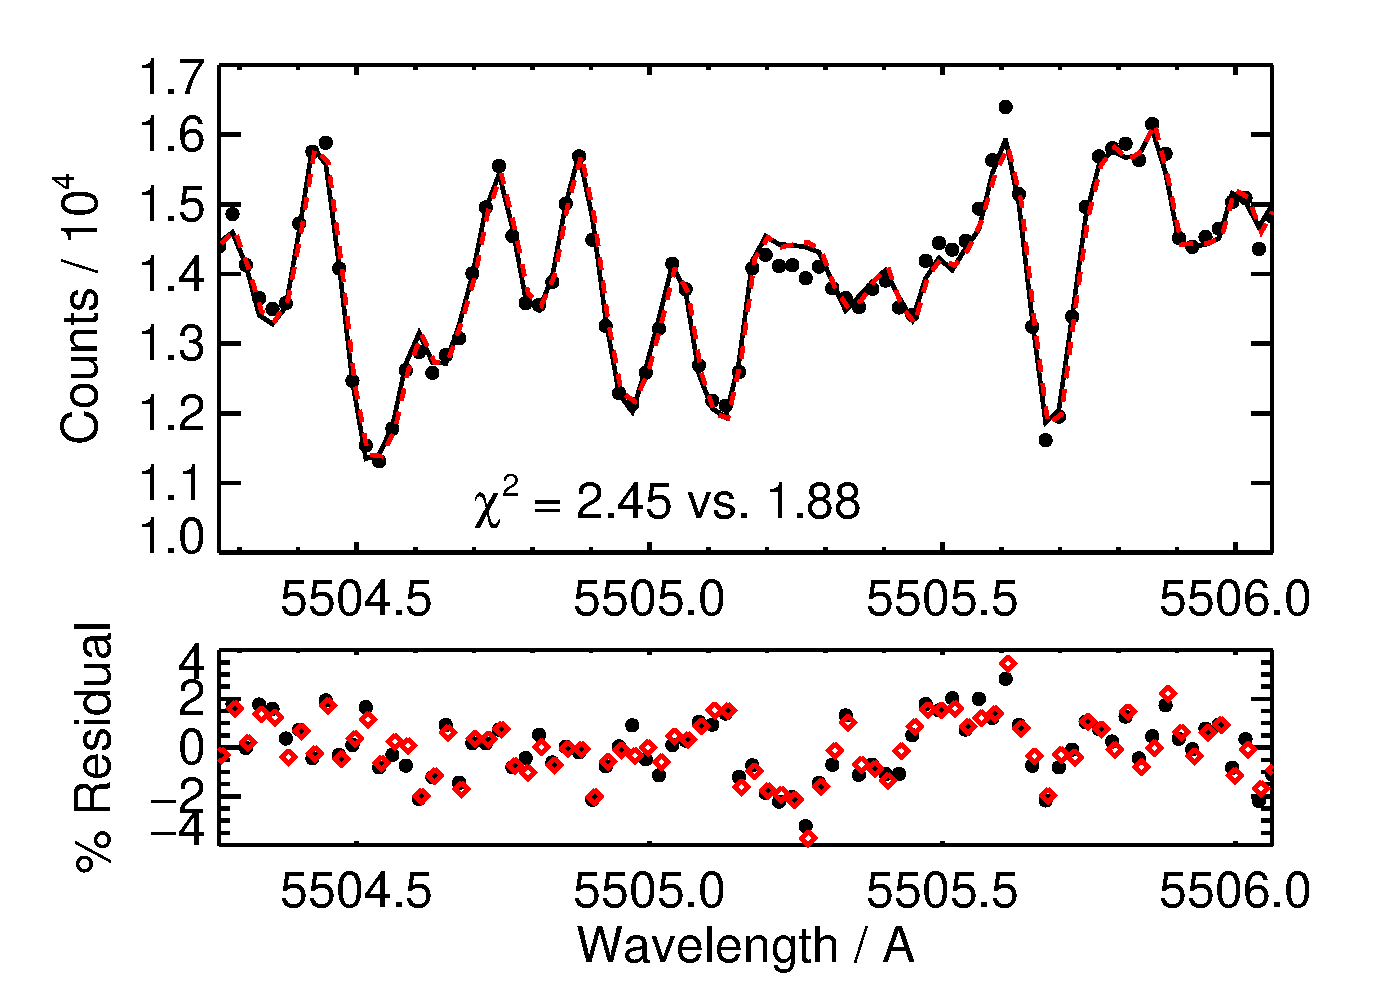
\includegraphics[scale=0.35]{het/20120124.176005.chunk191.compfit.eps}}
\caption{Introducing a sharp feature into the \het\ IP model, a
  triangle on top of the GH IP (red curve in the left panel), produces
  a better fit, somewhat to our surprise. The black in the left panel
  is the best-fit GH IP. GH$+$triangle is the IP model that produces
  the least $\chi^2_\nu$ among all of our IP models. However, as shown
  by the right panel, the two fits barely have any visible difference
  (red curve for GH$+$triangle IP and black for GH; bottom panel plots
  the residuals). Such a sharp feature in the IP is unphysical, and we
  interpretate this results as a hint for an unreliable iodine atlas
  (the sharp peak at the center is perhaps the IP model trying to
  ``stretch" the iodine lines deeper; see Section~\ref{het:sec:fts}
  for more details).
\label{het:fig:iodipcomp}}
\end{figure}
%----------------------------------------------------------------



To end this section with a positive note, we present a promising lead
for a better IP function for \hrs, the modified Moffat function:
\begin{equation}
[1+(x/\theta)^2]^{-\beta\cdot(x/\delta)^2}
\end{equation} 
It is called the ``modified" Moffat function because the original
Moffat function does not have the $(x/\delta)^2$ term. We added this
term to add flexibility at the wings to enable change of characteristic
IP width while preserving wing profile. Figure~\ref{het:fig:moffat}
illustrates the results using the modified Moffat fitting a ThAr line
(insert), and also the $\chi^2_\nu$ distribution of all spectral
chunks for this new IP compared with the GH IP. 

This modified Moffat function is potentially applicable to other
fiber-fed instruments, since these instruments tend to have IPs with
the same characteristic flat top and sharp wings.

One can image getting a better fit by adding small perturbation terms to the
modified Moffat IP to account for IP asymmetry and subtle wings due to
scattered light. However, getting a better fit to the iodine lines means
disentangling the effects of a bad IP model and a ``bad iodine atlas''
or modeling a changing cell, which could be challenging.



%----------------------------------------------------------------
% Fitting with a Moffat function
% plot made by ~/ExoPlanet-2010-2011/HET-HRS-IP/06-line_through_dots/thar.pro
% and stored in ./plots/
\begin{figure}
\centering
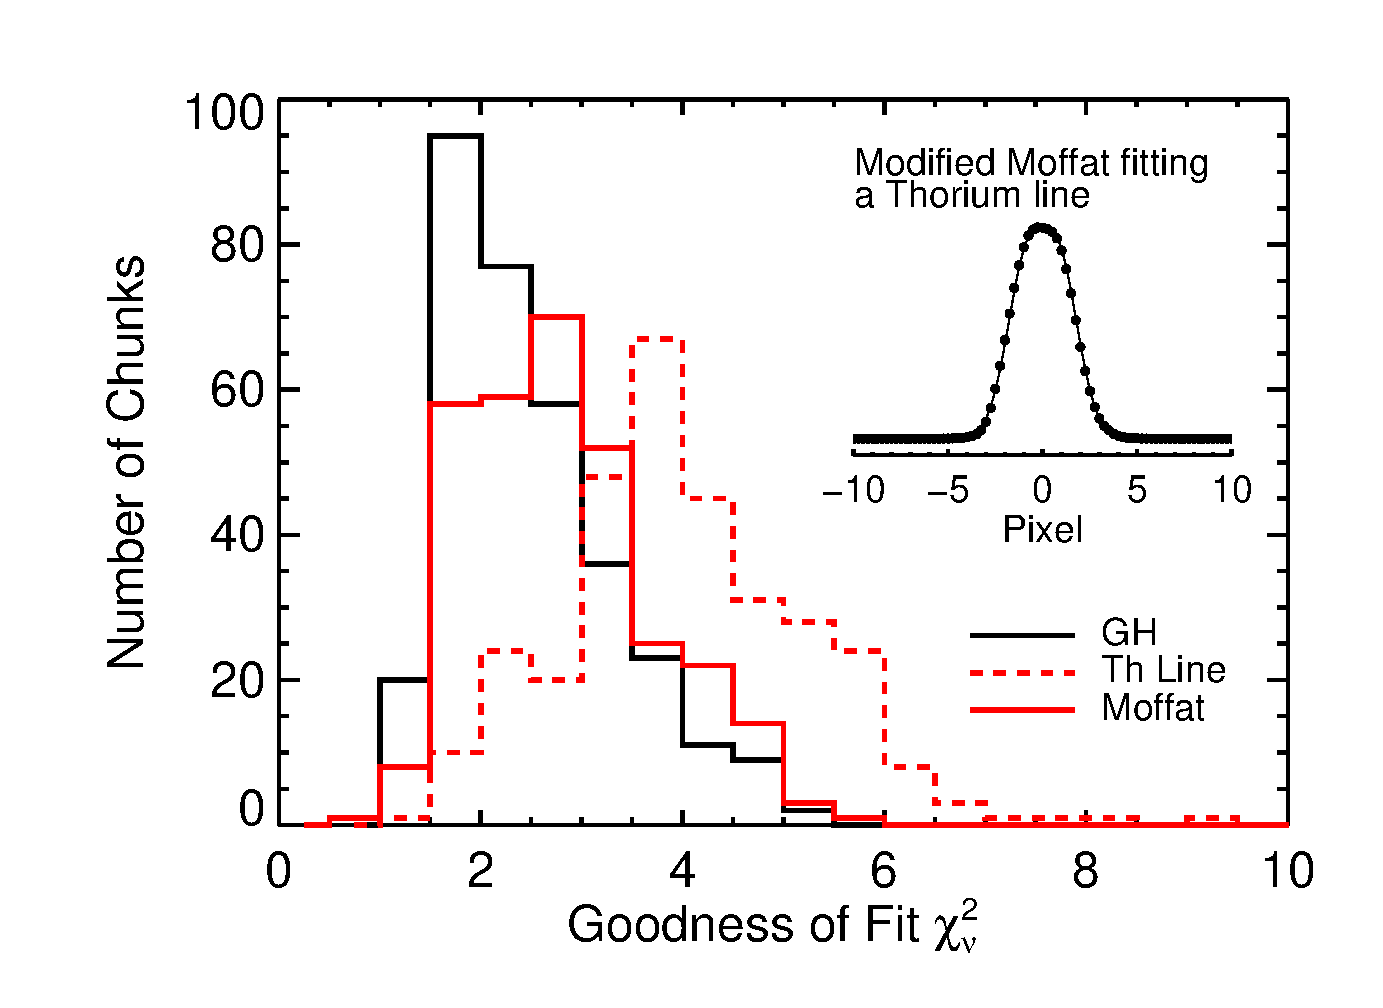
\includegraphics[scale=0.45]{het/thar_vs_moffat.eps}
\caption{Histogram of goodness of fit, $\chi^2_\nu$, values for
  spectral chunks of an iodine spectrum. The modified Moffat function
  (red) performs almost equally well while having only 3 parameters,
  com- pared with the complicated 11-parameter GH function (black
  solid). Red dashed histogram is for fits using a ThAr line profile
  as IP. The insert is showing the modified Moffat function can fit a
  ThAr line quite well.
\label{het:fig:moffat}}
\end{figure}
%----------------------------------------------------------------


